\section{VC Dimensions}
\label{sec:vc}

\begin{enumerate}
\item Consider learning problems where examples are points in the two
  dimensional plane. What is the VC dimension of the following concept
  classes? (In each case you need to prove your answer by showing both
  the upper and lower bounds.)

  \begin{enumerate}
    
  \item \relax[15 points] The concept class $H_c$ consisting of
    circles, with points strictly outside being negative.


  \item ~[15 points] The concept class $H$ is defined as follows: A
    function $h \in H$ is specified by two parameters $a$ and
    $b$. An example ${\bf x} = \{x_1, x_2\}$ in $\Re^2$ is labeled
    as $+$ if and only if $x_1 \geq a$ and $x_2 \leq b$ and is
    labeled $-$ otherwise.

    For example, if we set $a = 1, b = 4$, the grey region in figure
    \ref{f1} is the region of ${\bf x} = \{x_1, x_2\}$ that has label
    $+1$. 

    What is the VC dimension of this class?

    \begin{figure}[h]
      \centering
      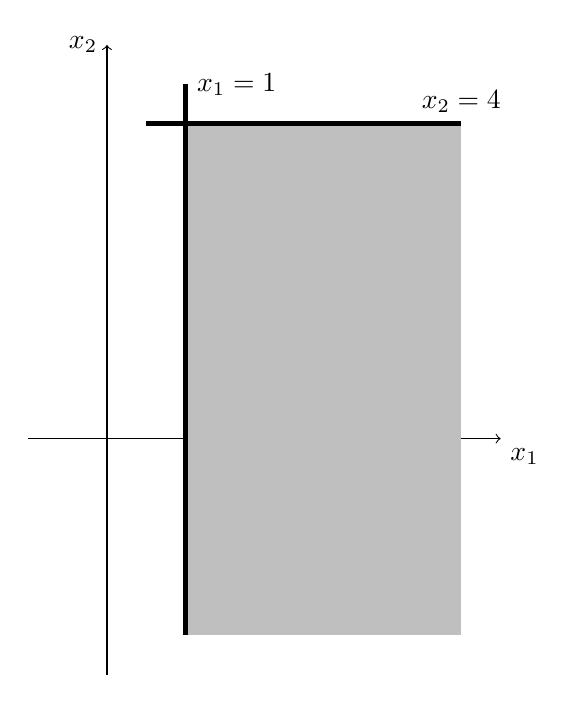
\begin{tikzpicture}[domain=0:2]
        \draw[->] (-1,0) -- (5,0) node[below right] {$x_1$};
        \draw[->] (0,-3) -- (0,5) node[left] {$x_2$};
        \fill[gray!50] (1,4) -- (1,-2.5) -- (4.5,-2.5) -- (4.5,4);
        \draw [ultra thick] (1,4.5) node [right] {$x_1 = 1$} -- (1,-2.5);
        \draw [ultra thick] (0.5,4) -- (4.5,4) node [above] {$x_2 = 4$};
      \end{tikzpicture}
      \caption{An example with $a = 1, b = 4$. All points in the gray region
        (extending infinitely) shows the region that will be labeled as
        positive.} \label{f1}
    \end{figure}

  \end{enumerate}



\item ~[{\bf For 6350 Students,} 15 points] Let two hypothesis classes
  $H_1$ and $H_2$ satisfy $H_1 \subseteq H_2$. Prove: $VC(H_1) \leq
  VC(H_2)$.
  
\end{enumerate}

%%% Local Variables:
%%% mode: latex
%%% TeX-master: "hw"
%%% End:
